\documentclass{article}
% Comment the following line to NOT allow the usage of umlauts
\usepackage[utf8]{inputenc}

\usepackage{amsfonts, amsthm, amsmath, braket} 
\usepackage{tikz}
\usetikzlibrary{angles, quotes, calc, patterns}
% Uncomment the following line to allow the usage of graphics (.png, .jpg)
%\usepackage{graphicx}


% Start the document
\begin{document}

% Create a new 1st level heading
\section{Main Heading}

For orthogonal
\[
c^2 = a^2 + b^2
\]

For any obtuse 

\[
c^2 = a^2 + b^2 + 2ad
\]

where d is b projected along a


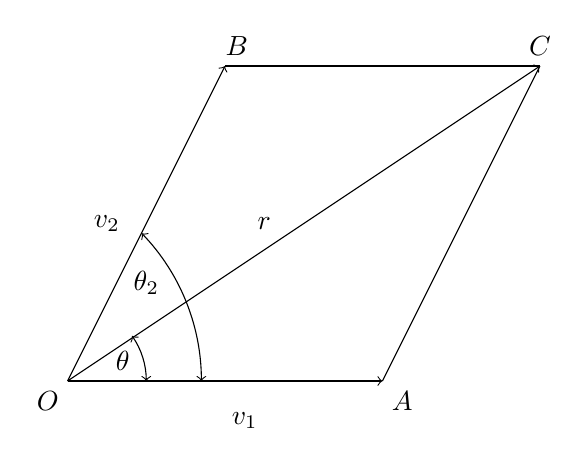
\begin{tikzpicture}
%the vectors
\draw [->, black] (1.0,0) -- (5.0,0.0);
\draw [black] (3.25, -0.5) node [black]{$v_1$};

\draw [->, black] (1.0,0) -- (3.0,4.0);
\draw (1.5, 2.0) node [black]{$v_2$}; 
\draw [black, <->] (2.7,0) arc (0:44:2.7); 
\draw (2., 1.25) node {$\theta_2$};

%the shadow
\draw [-, black] (5.0, 0,0) -- (7.0,4.0);
\draw [-, black] (3.0,4.0) -- (7.0,4.0);

%the resultant
\draw [->, black] (1.0,0) -- (7.0,4.0);
\draw [black] (3.5, 2.0) node [black]{$r$}; 
\draw [black, <->] (2.0,0) arc (0:35:1);
\draw (1.7, .25) node {$\theta$};

\draw [black] (.75, -.25) node {$O$}; 
\draw [black] (5.25, -.25) node {$A$}; 
\draw [black] (3.15, 4.25) node {$B$}; 
\draw [black] (7.0, 4.25) node {$C$}; 
\end{tikzpicture}
\begin{align*}
OA &= v_1/0 \\
OB &= v_2/\theta_2\\
OC &= r/\theta\\
r^2 &= v_1^2 + v_2^2 + 2v_1v_2\cos\theta\\
\tan\theta &= \frac{v_2\sin\theta_2}{v_1 + v_2\cos\theta_2};
\end{align*}
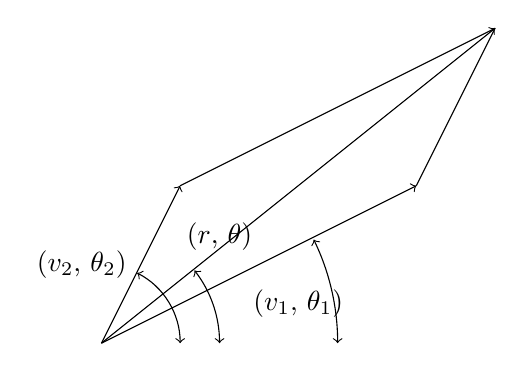
\begin{tikzpicture}
%the vectors
\draw [->, black] (1.0,0) -- (5.0,2.0);
\draw [dotted] (3.5, 0.5) node [black]{($v_1$, $\theta_1$)};
\draw [black, <->] (4.0,0) arc (0:26:3.0); 

\draw [->, black] (1.0,0) -- (2.0,2.0);
\draw [dotted] (.75, 1.) node [black]{($v_2$, $\theta_2$)};
\draw [black, <->] (2.0,0) arc (0:63:1.); 

%the shadow
\draw [-, black] (5.0, 2,0) -- (6.0,4.0);
\draw [-, black] (2.0,2.0) -- (6.0,4.0);
%the resultant
\draw [->, black] (1.0,0) -- (6.0,4.0);
\draw [dotted] (2.5, 1.35) node [black]{($r$, $\theta$)};
\draw [black, <->] (2.5,0) arc (0:38:1.5); 
\end{tikzpicture}

% Uncomment the following two lines if you want to have a bibliography
%\bibliographystyle{alpha}
%\bibliography{document}

\end{document}
